\begin{center}
\Huge
Vektorregning
\end{center}

\section*{Vektorrepræsentation}
\stepcounter{section}
Vi vil til at starte med definere, hvad vi mener med en vektor.
\begin{defn}[Vektor]
	En vektor $\vv{v}$ er et objekt med to koordinater $v_1$ og $v_2$, der begge er tal. 
	Vi skriver vektoren op som
	\begin{align*}
		\vv{v} = 
		\begin{pmatrix}
		v_1 \\ v_2
		\end{pmatrix}.
	\end{align*}
\end{defn}
En vektor kan repræsenteres i et koordinatsystem som en pil. Vi vil typisk starte pilen i origo (husk, at origo er punktet $(0,0)$ i et koordinatsystem), men vi kan i princippet placere den hvor vi vil. På Figur \ref{fig:vektorrep} kan vi se, hvordan vi kan tegne en vektorrepræsentant.

\begin{figure}[H]
	\centering
	\begin{tikzpicture}
		\begin{axis}[
			axis lines = middle, 
			xmin = -2, xmax = 8,
			ymin = -2, ymax = 8,
			x = 1cm, y = 1cm, 
			ticks = none,
			xlabel = $x$, ylabel = $y$,
		]
			\draw[-{Stealth[scale=1.5]}, thick, color = teal] (axis cs: 2,1) -- 
			(axis cs: 6,7) node[midway, xshift = -5pt, yshift = 5pt, color = teal] {$\vv{v}$};
			\draw[color = purple, dashed, thick] (axis cs: 2,1) -- (axis cs: 6,1); 
			\draw[color = purple, dashed, thick] (axis cs: 6,7) -- (axis cs: 6,1); 
			\draw [decorate,decoration={brace,amplitude=5pt,mirror,raise=1ex}, color = purple]
  			(axis cs: 2,1) -- (axis cs: 6,1) node[midway,yshift=-1.5em] {$v_1$};
  			\draw [decorate,decoration={brace,amplitude=5pt,raise=1ex}, color = purple]
 			(axis cs: 6,7) -- (axis cs: 6,1) node[midway,xshift=1.5em] {$v_2$};
		\end{axis}
	\end{tikzpicture}	
	\caption{Repræsentant for en vektor}
	\label{fig:vektorrep}
\end{figure}

\begin{exa}
	\label{exa:vektorrep}
	Vi har to vektorer $\vv{u}$ og $\vv{v}$ givet ved
	\begin{align*}
		\vv{u} &= 
		\begin{pmatrix}
			4 \\ 3
		\end{pmatrix}
		\\
		\vv{v} &=
		\begin{pmatrix}
			-2 \\ -5
		\end{pmatrix}
	\end{align*}
	På Figur \ref{fig:tovektorer} kan vi se en repræsentant for hver af disse vektorer
	\begin{figure}[H]
		\centering
		\begin{tikzpicture}
			\begin{axis}[
				axis lines = middle, 
				xmin = -2, xmax = 8,
				ymin = -2, ymax = 8,
				x = 1cm, y = 1cm,  
				xlabel = $x$, ylabel = $y$
			]
			%u
			\draw[-{Stealth[scale=1.5]}, thick, color = teal] (axis cs: 3,1) -- 
			(axis cs: 6,5) node[midway, xshift = -5pt, yshift = 5pt, color = teal] {$\vv{u}$};
			%v
			\draw[-{Stealth[scale=1.5]}, thick, color = olive] (axis cs: 3,7) -- 
			(axis cs: 1,2) node[midway, xshift = -5pt, yshift = 5pt, color = olive] {$\vv{v}					$};
			%u-dashes
			\draw[dashed, thick, color = teal] (axis cs: 3,1) -- (axis cs: 6,1) 
			node [midway, yshift = -9pt, color = teal] {$4$};
			\draw[dashed, thick, color = teal] (axis cs: 6,1) -- (axis cs: 6,5) 
			node [midway, xshift = 9pt, color = teal] {$3$};
			%v-dashes
			\draw[dashed, thick, color = olive] (axis cs: 1,2) -- (axis cs: 3,2) 
			node [midway, yshift = -9pt, color = olive] {$-2$};
			\draw[dashed, thick, color = olive] (axis cs: 3,2) -- (axis cs: 3,7) 
			node [midway, xshift = 9pt, color = olive] {$-5$};
			\end{axis}
		\end{tikzpicture}
		\caption{Repræsentanter for to vektorer}
		\label{fig:tovektorer}
	\end{figure}
\end{exa}

\section*{Sum, differens og skalering}	
\stepcounter{section}

Vi starter med at definere, hvordan vi geometrisk lægger to vektorer sammen. Hvis vi ønsker at lægge to vektorer $\vv{u}$ og $\vv{v}$ sammen, så sætter vi deres repræsentanter i forlængelse af hinanden og danner en ny vektor $\vv{u} + \vv{v}$ fra begyndelsen af den første vektor til enden af den anden vektor. 

\begin{exa}
	Vi ønsker at lægge vektorerne $\vv{u}$ og $\vv{v}$ fra Eksempel \ref{exa:vektorrep} sammen.
	Vi sætter derfor vektorerne i forlængelse af hinanden som vi kan se på Figur
	 \ref{fig:vektorsum}
	\begin{figure}[H]
		\centering
		\begin{tikzpicture}
			\begin{axis}[
				axis lines = middle, 
				xmin = -2, xmax = 8,
				ymin = -2, ymax = 8,
				x = 1cm, y = 1cm,  
				xlabel = $x$, ylabel = $y$
			]
			%u
			\draw[-{Stealth[scale=1.5]}, thick, color = teal] (axis cs: 3,1) -- 
			(axis cs: 6,5) node[midway, xshift = -5pt, yshift = 5pt, color = teal] {$\vv{u}$};
			%v
			\draw[-{Stealth[scale=1.5]}, thick, color = olive] (axis cs: 6,5) -- 
			(axis cs: 4,0) node[midway, xshift = 5pt, yshift = -5pt, color = olive] {$\vv{v}					$};
			\draw[-{Stealth[scale=1.5]}, thick, color = purple] (axis cs: 3,1) -- 
			(axis cs: 4,0) node[midway, xshift = -15pt, yshift = -8pt, color = purple]
			 {$\vv{u} + \vv{v}$};
			
			\end{axis}
		\end{tikzpicture}
		\caption{Sum af to vektorer}
		\label{fig:vektorsum}
	\end{figure}
\end{exa}
Skal vi trække en vektor $\vv{u}$ fra en vektor $\vv{v}$, så skal vi vende repræsentanten for $\vv{u}$ om og derefter lægge vektorerne sammen.

\begin{exa}
	Har vi to vektorer $\vv{u}$ og $\vv{v}$ givet ved
	\begin{align*}
		\vv{u} &=
		\begin{pmatrix}
			2 \\ 3
		\end{pmatrix} \\
		\vv{v} &=
		\begin{pmatrix}
			3 \\ -4
		\end{pmatrix}
	\end{align*}
	På Figur \ref{fig:vektordif} kan vi se, hvordan vi trækker $\vv{u}$ fra $\vv{v}$
	\begin{figure}[H]
		\centering
		\begin{tikzpicture}
			\begin{axis}[
				axis lines = middle, 
				xmin = -5, xmax = 8,
				ymin = -5, ymax = 8,
				x = 1cm, y = 1cm, 
				xlabel = $x$, ylabel = $y$
			]
			%u
			\draw[-{Stealth[scale=1.5]}, thick, color = teal] (axis cs: -3,0) -- 
			(axis cs: -1,3) node[midway, xshift = -5pt, yshift = 5pt, color = teal] 
			{$\vv{u}$};
			%v
			\draw[-{Stealth[scale=1.5]}, thick, color = olive] (axis cs: -3,0) -- 
			(axis cs: 0,-4) node[midway, xshift = -5pt, yshift = -5pt, color = olive] {$\vv{v}					$};
			\draw[-{Stealth[scale=1.5]}, thick, color = teal] (axis cs: 2,-2) -- 
			(axis cs: 4,1) node[midway, xshift = 5pt, yshift = -5pt, color = teal] {$\vv{u}$};
			\draw[-{Stealth[scale=1.5]}, thick, color = olive] (axis cs: 4,1) -- 
			(axis cs: 1,5) node[midway, xshift = 7pt, yshift = 7pt, color = olive] {$\vv{-v}					$};
			Z
			\draw[-{Stealth[scale=1.5]}, thick, color = purple] (axis cs: 2,-2) -- 
			(axis cs: 1,5) node[midway, xshift = -18pt, yshift = -10pt, color = purple] 
			{$\vv{u}-\vv{v}$};
			\end{axis}
		\end{tikzpicture}
		\caption{Differens af to vektorer}
		\label{fig:vektordif}
	\end{figure}
\end{exa}

Ganger vi en vektor med et tal, så gør vi den tilsvarende længere.
\begin{exa}
	En vektor $\vv{u}$ er givet ved
	\begin{align*}
		\vv{u} = 
		\begin{pmatrix}
			1 \\ 3
		\end{pmatrix}
	\end{align*}
	På Figur \ref{fig:vektorskalering} kan vi se vektorerne $\vv{u}$, $2\vv{u}$ og $-\vv{u}$.
	\begin{figure}[H]
		\centering
		\begin{tikzpicture}
			\begin{axis}[
				axis lines = middle, 
				xmin = -5, xmax = 8,
				ymin = -5, ymax = 8,
				x = 1cm, y = 1cm, 
				xlabel = $x$, ylabel = $y$
			]
			%u
			\draw[-{Stealth[scale=1.5]}, thick, color = teal] (axis cs: -2,1) -- 
			(axis cs: -1,4) node[midway, xshift = -5pt, yshift = 5pt, color = teal] 
			{$\vv{u}$};
			%v
			\draw[-{Stealth[scale=1.5]}, thick, color = teal] (axis cs: 1,1) -- 
			(axis cs: 3,7) node[midway, xshift = 10pt, yshift = -5pt, color = teal] {$2\vv{u}					$};
			\draw[-{Stealth[scale=1.5]}, thick, color = teal] (axis cs: -1,-1) -- 
			(axis cs: -2,-4) node[midway, xshift = -13pt, yshift = -5pt, color = teal] {$-\vv{u}$};
			\end{axis}
		\end{tikzpicture}
		\caption{Skalering af vektorer}
		\label{fig:vektorskalering}
	\end{figure}
\end{exa}

\newpage
\subsection*{Opgave 1}

Tegn følgende vektorer i koordinatsystemet

\begin{align*}
	&\vv{a} =
	\begin{pmatrix}
		2 \\ 3
	\end{pmatrix}
	&
	&\vv{b} = 
	\begin{pmatrix}
		4 \\ -2
	\end{pmatrix} 
	&	
	&\vv{c} =
	\begin{pmatrix}
		-5 \\ -2
	\end{pmatrix}
	\\
	&\vv{d} = 
	\begin{pmatrix}
		-1 \\ 6
	\end{pmatrix}
	&
	&\vv{e} = 
	\begin{pmatrix}
		7 \\ -2
	\end{pmatrix}
	&
	&\vv{f} = 
	\begin{pmatrix}
		5 \\ 3
	\end{pmatrix}
\end{align*}
\begin{center}
		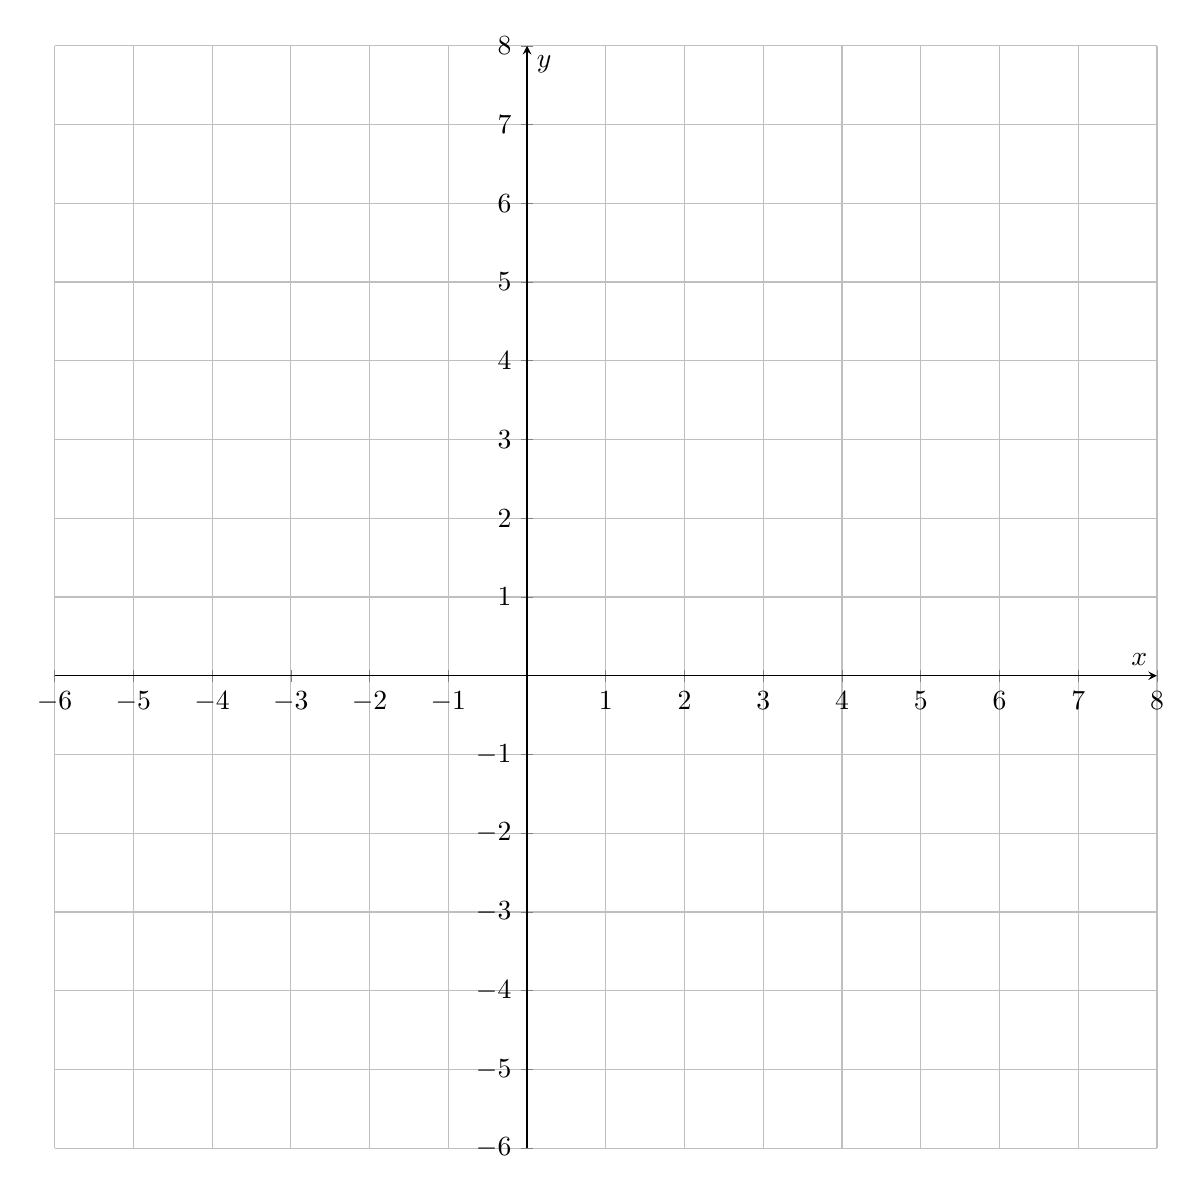
\begin{tikzpicture}
			\begin{axis}[
				axis lines = middle, 
				xmin = -6, xmax = 8,
				ymin = -6, ymax = 8,
				x = 1cm, y = 1cm, 
				xlabel = $x$, ylabel = $y$,
				grid				
			]
			\end{axis}
		\end{tikzpicture}
\end{center}
\newpage

\subsection*{Opgave 2}
Aflæs koordinaterne for følgende vektorer
\begin{center}
		\begin{tikzpicture}
			\begin{axis}[
				axis lines = middle, 
				xmin = -6, xmax = 8,
				ymin = -6, ymax = 8,
				x = 1cm, y = 1cm, 
				xlabel = $x$, ylabel = $y$,
				grid				
			]
			\draw[-{Stealth[scale=1.5]}, thick, color = teal] (axis cs: -2,1) -- 
			(axis cs: -1,4);
			\draw[-{Stealth[scale=1.5]}, thick, color = teal] (axis cs: 6,-2) -- 
			(axis cs: 1,1);
			\draw[-{Stealth[scale=1.5]}, thick, color = teal] (axis cs: 7,-1) -- 
			(axis cs: 4,-6);
			\draw[-{Stealth[scale=1.5]}, thick, color = teal] (axis cs: -5,-3) -- 
			(axis cs: -2,-6);
			\draw[-{Stealth[scale=1.5]}, thick, color = teal] (axis cs: -5,2) -- 
			(axis cs: -3,3);
			\draw[-{Stealth[scale=1.5]}, thick, color = teal] (axis cs: -5,3) -- 
			(axis cs: -4,6);
			\draw[-{Stealth[scale=1.5]}, thick, color = teal] (axis cs: 3,5) -- 
			(axis cs: 5,7);
			\draw[-{Stealth[scale=1.5]}, thick, color = teal] (axis cs: 1,7) -- 
			(axis cs: -2,-5);
			\end{axis}
		\end{tikzpicture}
\end{center}

\newpage

\subsection*{Opgave 3}

Bestem følgende summer af vektorer ved at tegne dem på koordinatsystemet og aflæs derefter deres koordinater

\begin{align*}
	&a) \
	\begin{pmatrix}
		2 \\ 2
	\end{pmatrix} + 
	\begin{pmatrix}
		-1 \\ 3
	\end{pmatrix}
	&
	&b) \
	\begin{pmatrix}
		-4 \\ -3
	\end{pmatrix} + 
	\begin{pmatrix}
		6 \\ -2
	\end{pmatrix}
	\\
	&c) \
	\begin{pmatrix}
		0 \\ 5
	\end{pmatrix} + 
	\begin{pmatrix}
		5 \\ 0
	\end{pmatrix}
	&
	&d) \ 
	\begin{pmatrix}
		-3 \\ 7
	\end{pmatrix} + 
	\begin{pmatrix}
		4 \\ -1
	\end{pmatrix}
\end{align*}

\begin{center}
		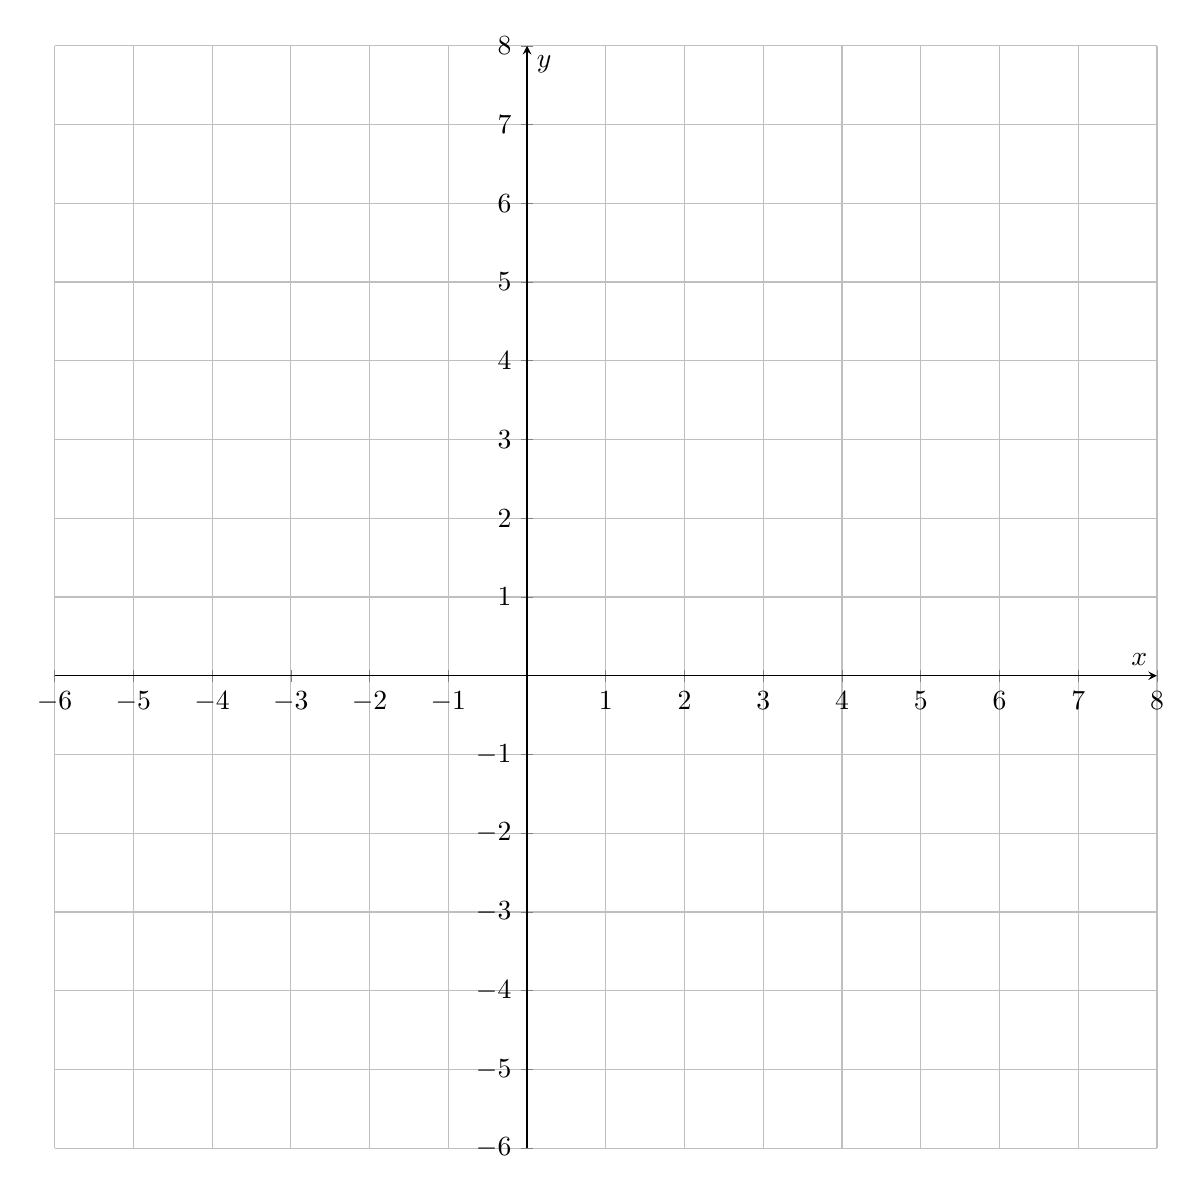
\begin{tikzpicture}
			\begin{axis}[
				axis lines = middle, 
				xmin = -6, xmax = 8,
				ymin = -6, ymax = 8,
				x = 1cm, y = 1cm, 
				xlabel = $x$, ylabel = $y$,
				grid				
			]
			\end{axis}
		\end{tikzpicture}
\end{center}

\subsection*{Opgave 4}
Bestem følgende differenser af vektorer ved at tegne dem i koordinatsystemet og aflæs derefter deres koordinater

\begin{align*}
	&a) \
	\begin{pmatrix}
		1 \\ 5
	\end{pmatrix} -
	\begin{pmatrix}
		-2 \\ 2
	\end{pmatrix}
	&
	&b) \
	\begin{pmatrix}
		2 \\ 1
	\end{pmatrix} + 
	\begin{pmatrix}
		-4 \\ 5
	\end{pmatrix}
	\\
	&c) \
	\begin{pmatrix}
		0 \\ 5
	\end{pmatrix} + 
	\begin{pmatrix}
		5 \\ 0
	\end{pmatrix}
	&
	&d) \ 
	\begin{pmatrix}
		1 \\ -2
	\end{pmatrix} + 
	\begin{pmatrix}
		0 \\ -3
	\end{pmatrix}
\end{align*}

\begin{center}
		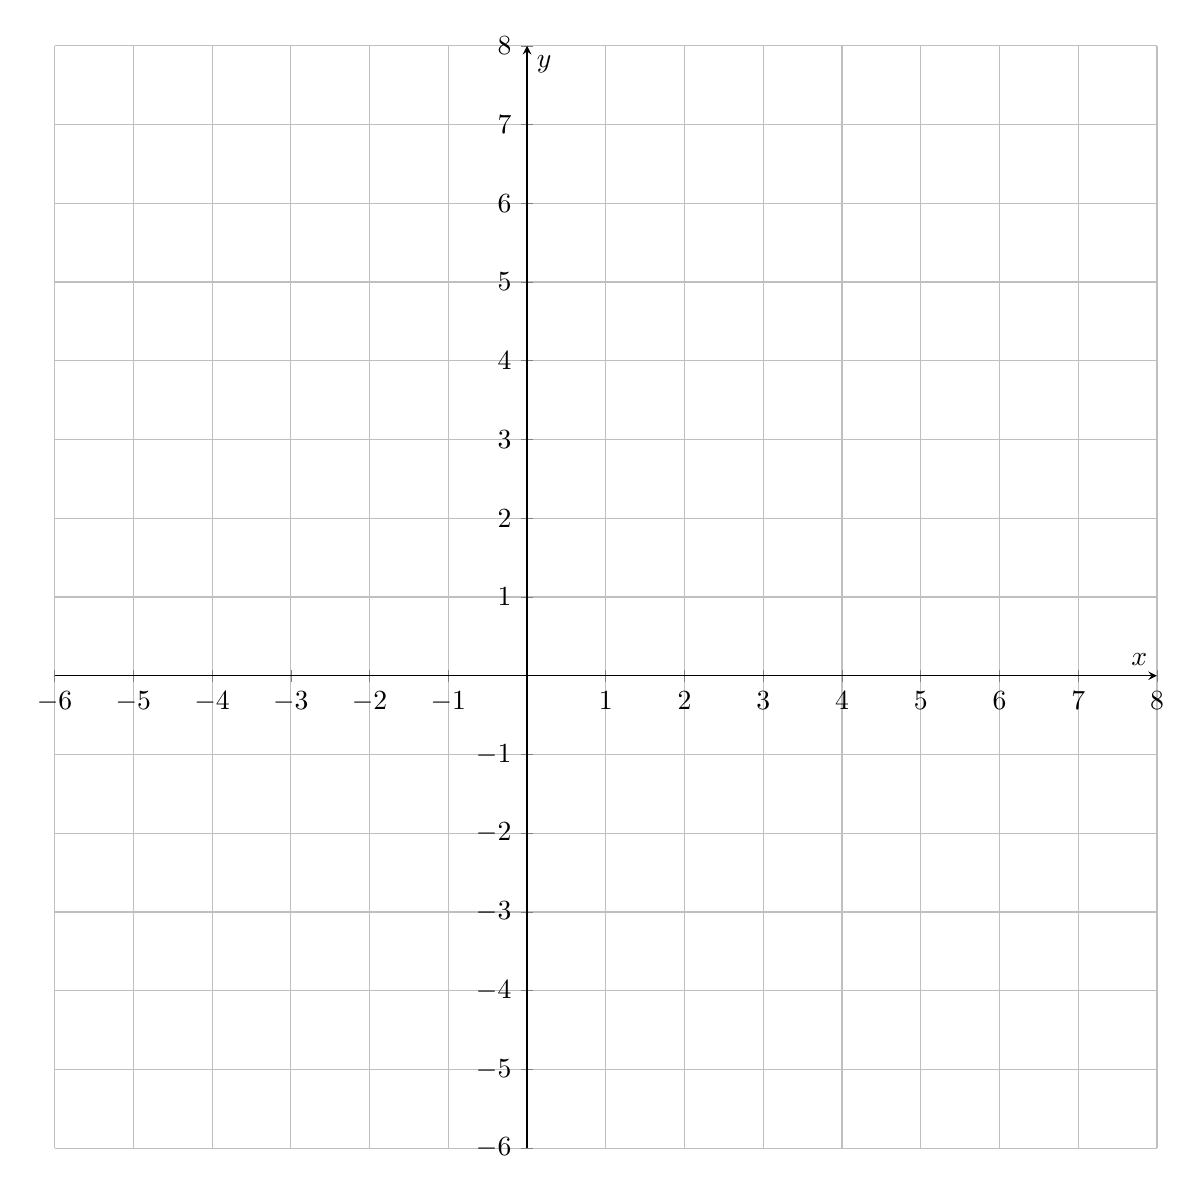
\begin{tikzpicture}
			\begin{axis}[
				axis lines = middle, 
				xmin = -6, xmax = 8,
				ymin = -6, ymax = 8,
				x = 1cm, y = 1cm, 
				xlabel = $x$, ylabel = $y$,
				grid				
			]
			\end{axis}
		\end{tikzpicture}
\end{center}

\newpage

\subsection*{Opgave 5}

For $\vv{u}$ og $\vv{v}$ givet ved
\begin{align*}
	&\vv{u} = 
	\begin{pmatrix}
		2 \\ -1
	\end{pmatrix} & 
	\vv{v} = 
	\begin{pmatrix}
		-3 \\ 3
	\end{pmatrix}
\end{align*}
tegn da vektorerne $\vv{u}$, $\vv{v}$, $-\vv{u}$, $2\vv{u}$, $3\vv{v}$ og $-\vv{v}$ og aflæs deres koordinater

\begin{center}
		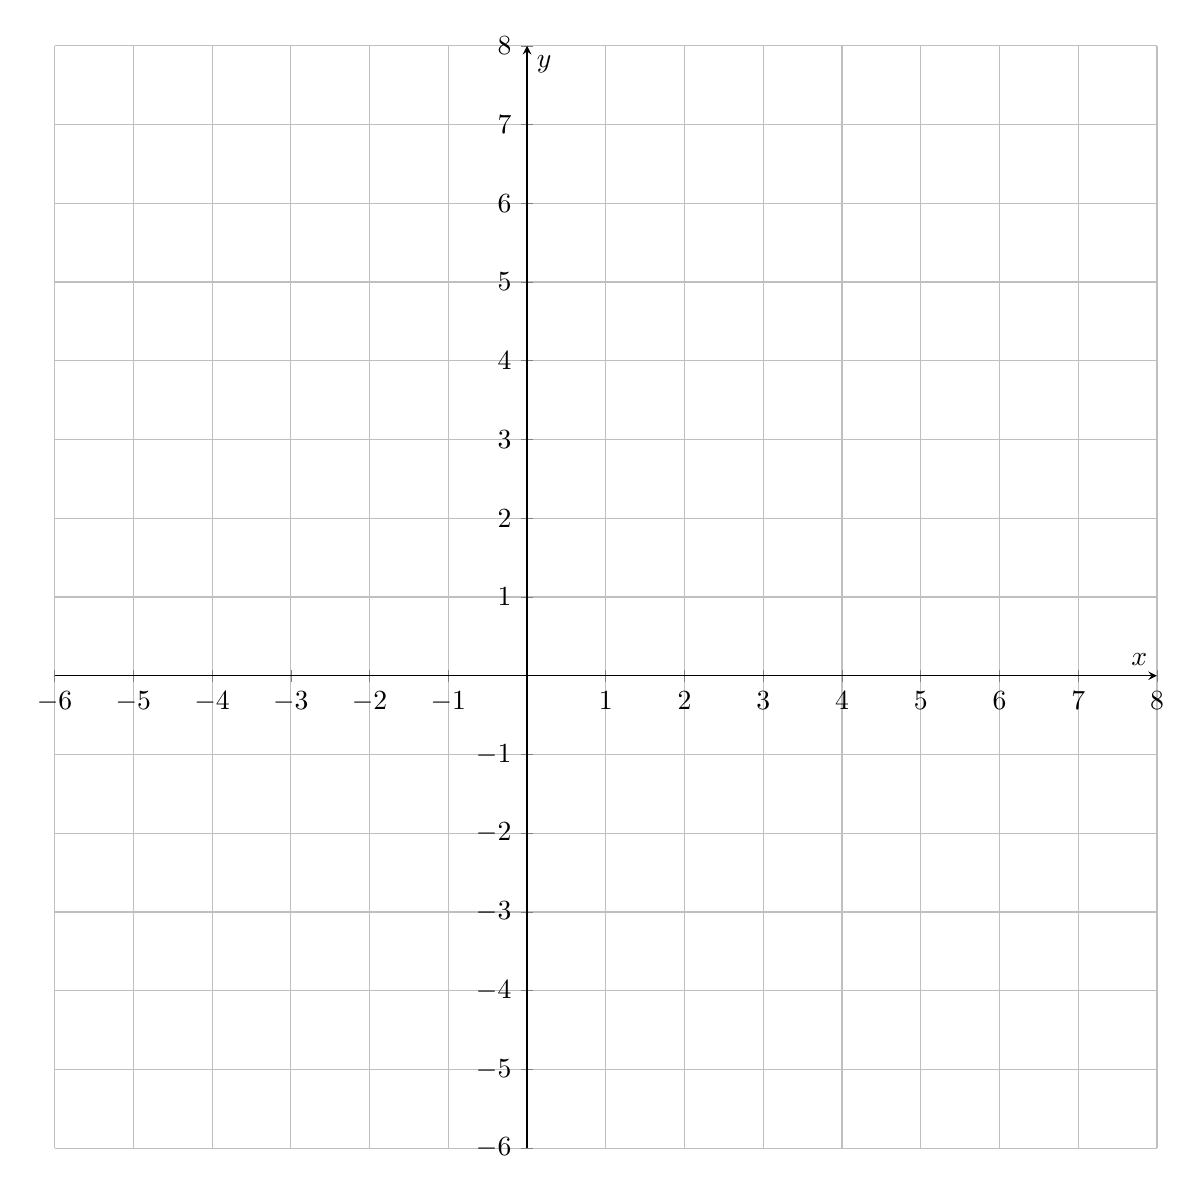
\begin{tikzpicture}
			\begin{axis}[
				axis lines = middle, 
				xmin = -6, xmax = 8,
				ymin = -6, ymax = 8,
				x = 1cm, y = 1cm, 
				xlabel = $x$, ylabel = $y$,
				grid				
			]
			\end{axis}
		\end{tikzpicture}
\end{center}

\newpage

\subsection*{Opgave 6}

Ved at betragte koordinaterne for summerne, differenserne og skaleringerne fra de tidligere opgaver, kan du så gennemskue, hvordan man laver disse operationer uden at tegne vektorerne men blot ved at anvende deres koordinater.

\subsection*{Opgave 7}
Fire vektorer er givet ved
\begin{align*}
	&\vv{a} = 
	\begin{pmatrix}
		4 \\ -3
	\end{pmatrix} 
	&
	&\vv{b} = 
	\begin{pmatrix}
		-2 \\ 5
	\end{pmatrix}
	\\
	&\vv{c} = 
	\begin{pmatrix}
		6 \\ 10
	\end{pmatrix}
	&
	&\vv{d} = 
	\begin{pmatrix}
		-11 \\ -7
	\end{pmatrix}
\end{align*}

\begin{enumerate}[label=\roman*)]
	\item Bestem $4\vv{a}$.
	\item Bestem $\vv{a} + \vv{b}$.
	\item Bestem $2\vv{b} - \vv{c}$.
	\item Bestem $\vv{a}+\vv{b}+\vv{c}+\vv{d}$.
	\item Bestem $-2\vv{d} - \vv{a}$.
	\item Bestem $\vv{a}-\vv{b}+\vv{c}-3\vv{d}$.
\end{enumerate}
